\documentclass[11pt]{article}
\usepackage[utf8]{inputenc}
\usepackage[margin=1in]{geometry}
\usepackage{amsmath, amssymb}
\usepackage{tikz}
\usetikzlibrary{arrows.meta, automata, positioning, calc, decorations.pathreplacing}
\usepackage{caption}

\title{Figures in TikZ: A Working Notebook}
\author{Razz}
\date{October 2026}

\begin{document}
\maketitle

These are the figures I keep redrawing. Each one lives in its own file under \texttt{figures/} so that it can be reused in a paper or a talk with a single \verb|\input|.

\section{A finite automaton}

Figure~\ref{fig:automaton} shows a deterministic automaton over $\{0, 1\}$ that accepts the binary strings whose value is divisible by three.

\begin{figure}[ht]
  \centering
  % Deterministic automaton for binary numbers divisible by three.
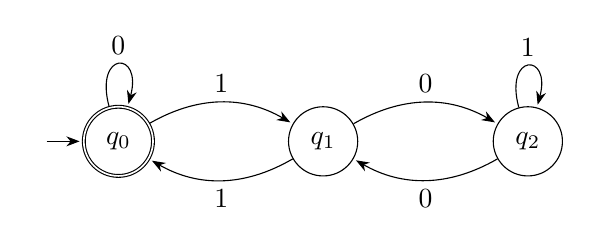
\begin{tikzpicture}[->, >=Stealth, shorten >=1pt, node distance=2.6cm, on grid, auto, initial text=]
  \node[state, initial, accepting] (q0) {$q_0$};
  \node[state] (q1) [right=of q0] {$q_1$};
  \node[state] (q2) [right=of q1] {$q_2$};
  \path
    (q0) edge [loop above] node {0} ()
    (q0) edge [bend left] node {1} (q1)
    (q1) edge [bend left] node {1} (q0)
    (q1) edge [bend left] node {0} (q2)
    (q2) edge [bend left] node {0} (q1)
    (q2) edge [loop above] node {1} ();
\end{tikzpicture}

  \caption{Divisibility by three. State $q_i$ means the prefix read so far is congruent to $i$ modulo 3.}
  \label{fig:automaton}
\end{figure}

\section{A small neural network}

\begin{figure}[ht]
  \centering
  % Fully connected network: 3 inputs, 4 hidden units, 2 outputs.
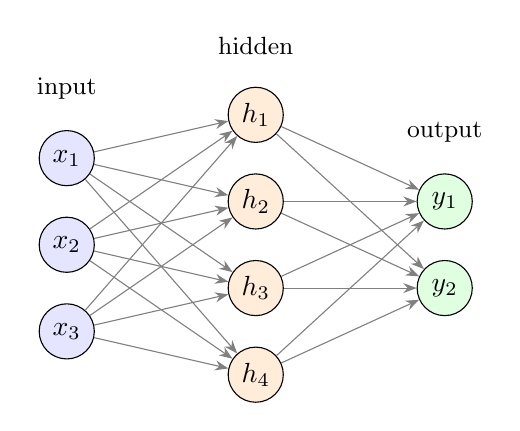
\begin{tikzpicture}[x=2.4cm, y=1.1cm, >=Stealth, neuron/.style={circle, draw, minimum size=7mm, inner sep=0pt}]
  \foreach \i in {1, 2, 3} {
    \node[neuron, fill=blue!10] (I\i) at (0, 2.5 - \i) {$x_\i$};
  }
  \foreach \j in {1, 2, 3, 4} {
    \node[neuron, fill=orange!15] (H\j) at (1, 3 - \j) {$h_\j$};
  }
  \foreach \k in {1, 2} {
    \node[neuron, fill=green!12] (O\k) at (2, 2 - \k) {$y_\k$};
  }
  \foreach \i in {1, 2, 3} {
    \foreach \j in {1, 2, 3, 4} {
      \draw[->, gray] (I\i) -- (H\j);
    }
  }
  \foreach \j in {1, 2, 3, 4} {
    \foreach \k in {1, 2} {
      \draw[->, gray] (H\j) -- (O\k);
    }
  }
  \node at (0, 2.3) {\small input};
  \node at (1, 2.8) {\small hidden};
  \node at (2, 1.8) {\small output};
\end{tikzpicture}

  \caption{A fully connected network with one hidden layer.}
  \label{fig:network}
\end{figure}

\section{A commutative diagram}

The universal property of the product $A \times B$:
\[
  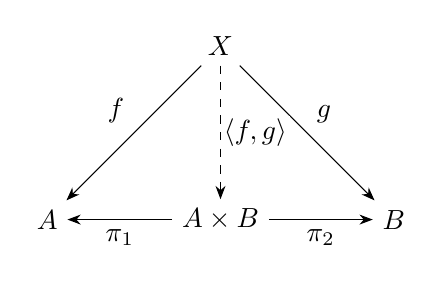
\begin{tikzpicture}[node distance=2.2cm, auto, >=Stealth]
    \node (X) {$X$};
    \node (P) [below of=X] {$A \times B$};
    \node (A) [left of=P] {$A$};
    \node (B) [right of=P] {$B$};
    \draw[->] (X) to node[swap] {$f$} (A);
    \draw[->] (X) to node {$g$} (B);
    \draw[->, dashed] (X) to node[fill=white, inner sep=1pt] {$\langle f, g \rangle$} (P);
    \draw[->] (P) to node {$\pi_1$} (A);
    \draw[->] (P) to node[swap] {$\pi_2$} (B);
  \end{tikzpicture}
\]

\section{Riemann sums}

\begin{figure}[ht]
  \centering
  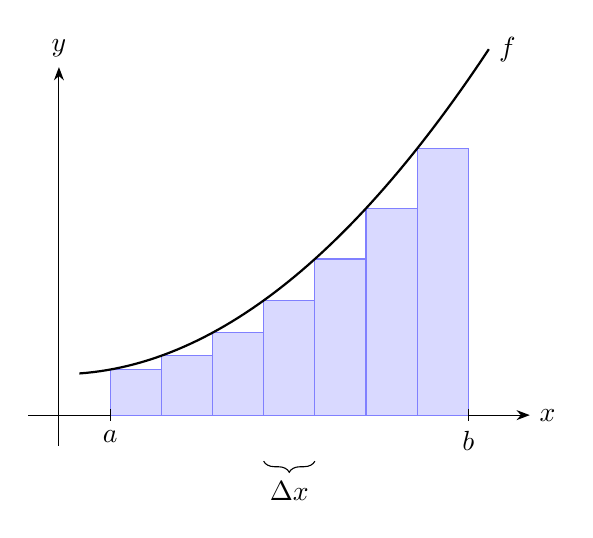
\begin{tikzpicture}[scale=1.3, >=Stealth]
    \draw[->] (-0.3, 0) -- (4.6, 0) node[right] {$x$};
    \draw[->] (0, -0.3) -- (0, 3.4) node[above] {$y$};
    \foreach \x in {0.5, 1.0, ..., 3.5} {
      \pgfmathsetmacro{\y}{0.18 * \x * \x + 0.4}
      \draw[fill=blue!15, draw=blue!50] (\x, 0) rectangle (\x + 0.5, \y);
    }
    \draw[thick, domain=0.2:4.2, samples=60] plot (\x, {0.18 * \x * \x + 0.4}) node[right] {$f$};
    \draw (0.5, 0.06) -- (0.5, -0.06) node[below] {$a$};
    \draw (4.0, 0.06) -- (4.0, -0.06) node[below] {$b$};
    \draw[decorate, decoration={brace, mirror, amplitude=4pt}] (2.0, -0.45) -- (2.5, -0.45) node[midway, below=4pt] {$\Delta x$};
  \end{tikzpicture}
  \caption{A left Riemann sum of $f$ on $[a, b]$ with seven subintervals.}
  \label{fig:riemann}
\end{figure}

\end{document}
